% exercise sheet with header on every page for math or close subjects
\documentclass[12pt]{article}
\usepackage[utf8]{inputenc} 
\usepackage{latexsym} 
\usepackage{multicol}
\usepackage{fancyhdr}
\usepackage{amsfonts} 
\usepackage{amsmath}
\usepackage{amssymb}
\usepackage{enumerate}
\usepackage{listings}
\usepackage{graphicx}
\usepackage{hyperref}

% Shortcuts for bb, frak and cal letters
\newcommand{\E}{\mathbb{E}}
\newcommand{\V}{\mathbb{V}}
\renewcommand{\P}{\mathbb{P}}
\newcommand{\N}{\mathbb{N}}
\newcommand{\R}{\mathbb{R}}
\newcommand{\C}{\mathbb{C}}
\newcommand{\Z}{\mathbb{Z}}
\newcommand{\Pfrak}{\mathfrak{P}}
\newcommand{\Pfrac}{\mathfrak{P}}
\newcommand{\Bfrac}{\mathfrak{P}}
\newcommand{\Bfrak}{\mathfrak{B}}
\newcommand{\Fcal}{\mathcal{F}}
\newcommand{\Ycal}{\mathcal{Y}}
\newcommand{\Bcal}{\mathcal{B}}
\newcommand{\Acal}{\mathcal{A}}
\newcommand{\intinfty}{\int^{\infty}_{-\infty}}

% formating
\topmargin -1.5cm 
\textheight 24cm
\textwidth 16.0 cm 
\oddsidemargin -0.1cm

% Fancy Header on every Page
\pagestyle{fancy}
\lhead{\textbf{Pattern and Speech Recognition}}
\rhead{Daniel Schäfer (2549458)\\ Christian Bohnenberger (2548364) \\ Dominik Weber (2548553)}
\renewcommand{\headrulewidth}{1.2pt}

\setlength{\headheight}{45pt} 

\begin{document}
\pagenumbering{gobble}

% TODO set the number of the exercise sheet here!
\setcounter{section}{9}
\setcounter{subsection}{0}


% ex 9.1
\subsection{ }


% ex 9.2
\subsection{ }

\underline{proof analogue to wikipedia:}\\\\

let $h$ be the convolution of $f$ and $f$:
$$ h(z) = \int^\infty_{-\infty} f(x)g(z-x) dx$$
$$\int \int \vert f(x)g(z-x) \vert dz dx = \int \vert f(x) \vert \int \vert g(z-x) \vert dz dx = \int \vert f(x) \vert \Vert g \Vert_1 dx = \Vert f \Vert_1 \Vert g \Vert_1$$

Hence by Fubinis Theorem we have that $h \in L^1(\R^n)$ so its Furioer transform H is defined by the integral formula
$$H(v) = \int^\infty_{-\infty} h(z)e^{-2 \pi i z v} dz$$
$$ \int^\infty_{-\infty} \int^\infty_{-\infty} f(x) f(z-x) dx e^{-2 \pi i z v} dz$$

$\vert f(x) g(z-x) e^{-2 \pi i z v} \vert = \vert f(x) g(z-x) \vert$ and we may apply Fubinis theorem again:

$$ H(v) = \int^\infty_{-\infty} f(x) (\int^\infty_{-\infty} g(z-x)e^{-2 \pi i z v} dz) dx$$

Now we substitute $y = z - x$ and $dy = dz$:
$$ H(v) = \intinfty f(x) ( \intinfty g(y)e^{-2 \pi i (y + x) v}dy)dx$$
$$ = \intinfty f(x) e ^{-2 \pi i x v} (\intinfty g(y) e ^{-2 x i y v}dy)dx$$
$$ = \intinfty f(x) e ^{-2 \pi x i v} dx \intinfty g(y)e^{-2 x i y v} dy$$

which are the definition of $F(v)$ and $G(v)$
$$ \ Rightarrow \quad H(v) = F(v) * G(v) $$




% ex 9.3
\subsection{ }



% ex 9.4
\subsection{ }
\begin{enumerate}[a)]
\item see code
\item split = 1: max = 246,pos:(134, 184)\\split = 2: max=[[ 234.  237.],[ 241.  246.]],pos=(127, 123)(29, 66)(11, 35)(6, 56)\\split = 4: max=[[ 228.  230.  231.  230.] [ 232.  234.  237.  237.] [ 241.  238.  246.  234.] [ 241.  238.  246.  207.]]pos=(51, 63)(53, 57)(33, 62)(31, 58)(39, 57)(63, 59)(29, 2)(7, 37)(11, 35)(63, 55)(6, 56)(22, 0)(9, 16)(63, 0)(6, 5)(61, 62)\\split=8:max=[[ 210.  219.  221.  221.  224.  224.  222.  221.] [ 222.  228.  229.  230.  231.  231.  230.  229.] [ 228.  231.  231.  233.  237.  236.  232.  231.] [ 231.  232.  232.  234.  236.  229.  237.  232.] [ 232.  232.  234.  234.  235.  223.  234.  232.] [ 241.  232.  235.  238.  246.  236.  234.  231.] [ 241.  232.  232.  238.  246.  123.  157.  134.] [ 211.  201.  232.  233.  231.  206.  182.  207.]]pos=(24, 29)(30, 31)(31, 29)(6, 29)(16, 30)(11, 31)(10, 30)(4, 31)(30, 29)(19, 31)(31, 25)(21, 25)(16, 31)(1, 30)(31, 26)(3, 28)(23, 31)(24, 15)(31, 15)(31, 29)(29, 2)(0, 1)(30, 29)(3, 11)(28, 25)(7, 25)(3, 11)(31, 27)(28, 1)(31, 1)(7, 5)(3, 5)(29, 12)(30, 0)(30, 7)(31, 5)(0, 5)(0, 12)(22, 0)(14, 0)(11, 3)(29, 12)(2, 7)(31, 23)(6, 24)(0, 18)(12, 12)(4, 1)(9, 16)(25, 1)(30, 1)(31, 0)(6, 5)(22, 3)(3, 0)(18, 18)(8, 1)(31, 26)(30, 0)(16, 0)(1, 2)(28, 31)(2, 29)(29, 30)
 \item s
\item d
\end{enumerate}


% ex 9.5
\subsection{ }

\textbf{Transfer Learning}:\\
The reason people usually use Transfer learning is because one rarely has a dataset of sufficient size to train a CNN from scratch! In practice it is common to pretrain a CNN on a very large Datatset and use this either as initialization or a fixed feature extractor for the task of interest.


% ex 9.5
\subsection{ }
\begin{enumerate}[a)]
    \item 
        A simple CNN for the CIFAR-10 classification task could look like this:
        $$ \text{Input Layer} \Rightarrow \text{Convolution Layer} \Rightarrow \text{RELU Layer} \Rightarrow \text{Pooling Layer} \Rightarrow \text{FC Layer}$$

        \begin{itemize}
            \item 
                The Input Layer will contain the R, G and B values of the 32 x 32 Image. 
            \item
                The Convolutional Layer will compute the output of neurons that are connected to local regions in the input, each computing the dot product between their weigts and a small region they are connected to in the input volume. This results for 32x32x8 if we decide to use 8 filters.
            \item
                The RELU Layer will apply an elementwise activation function, leaves the size of the colume unchanged
            \item
                The Pooling Layer will perform downsampling along the height and width resulting in for example a 16x16x8 volume
            \item
                The fully-connected Layer will compute the class scores, resulting in volumes of 1x1x10 which each of the 10 numbers being a score for one of the 10 classes.
        \end{itemize}
    \item
    	Backpropagation contains 2 steps. First the Propagation step here, we run the network with training examples to receive the predicted output of the network. \\
    	In the next step we can compute the error between the predicted outcome and the original value. In our case we use mean-squared error to do this.\\
    	These errors (we use multiple training examples) are used to calculate the gradient of the loss function as we did it every times before in the lecture.\\
    	These gradients are computed with respect to the weigths. This graident is used to update the weigths of the complete network by substracting a percentage of the gradient from every weight. This percentage is defined by the learning rate which has already been discussed in the lecture.
    	\newpage
	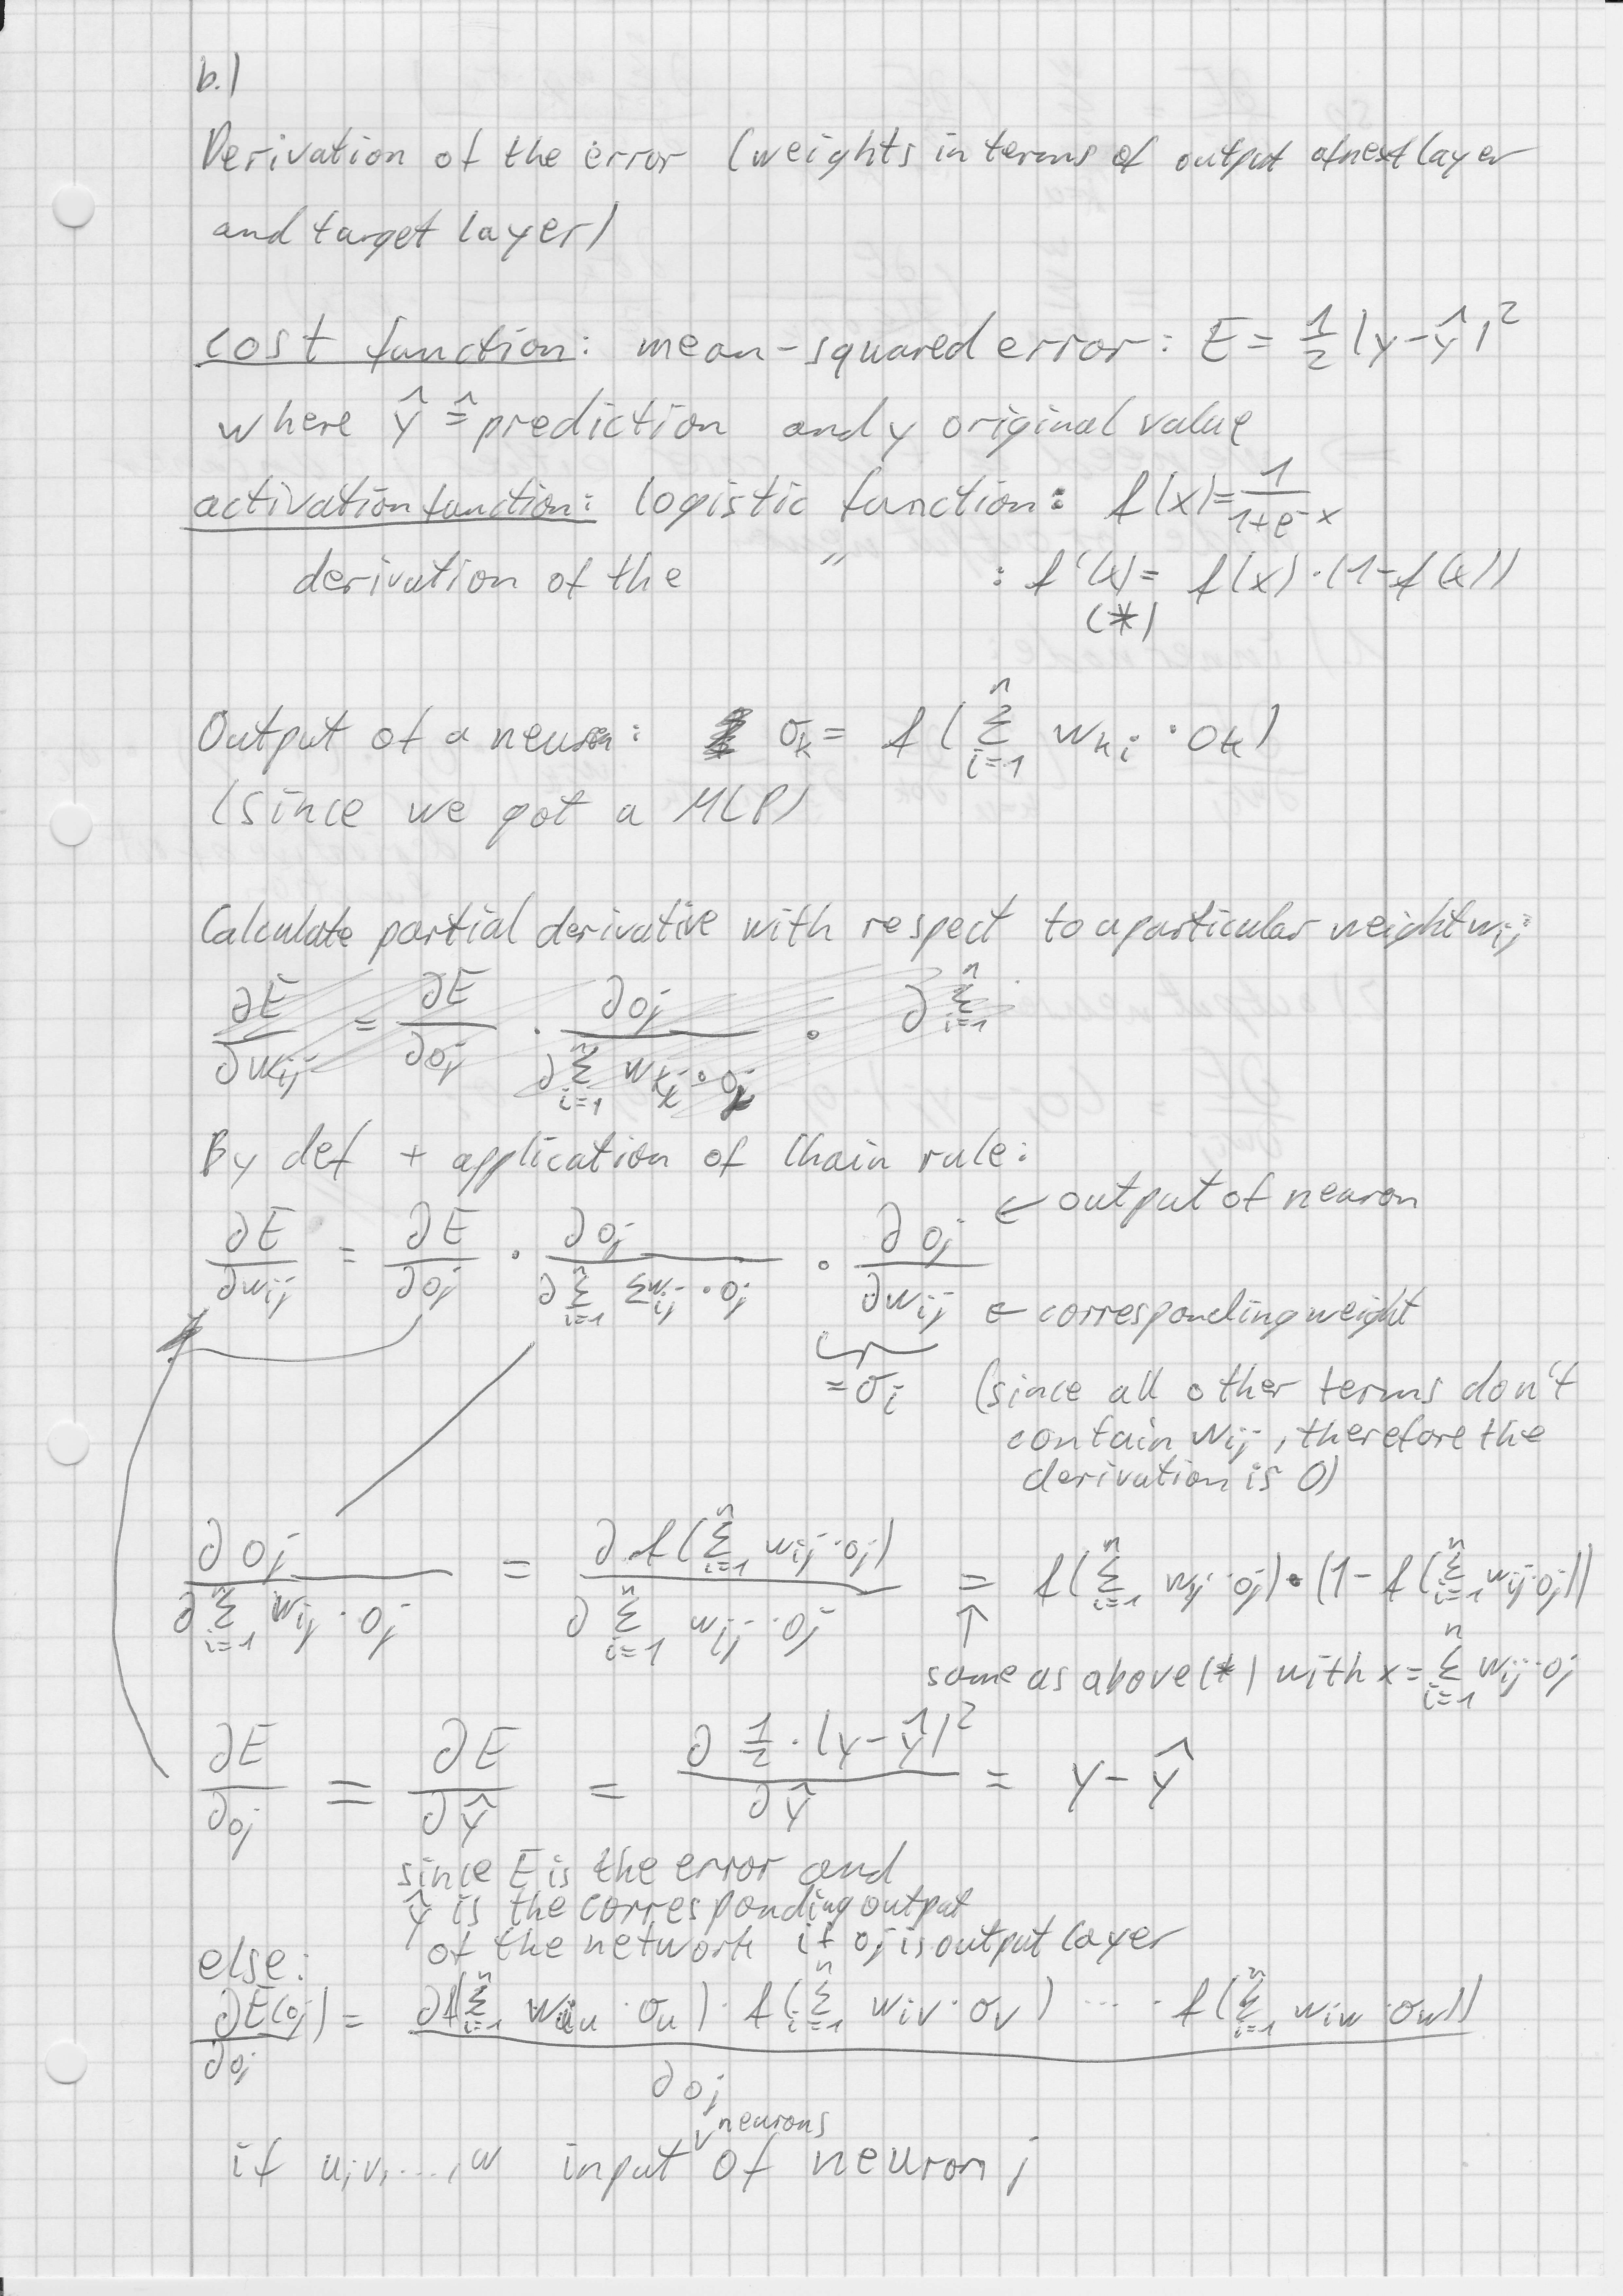
\includegraphics[scale = 0.1]{pictures/SCN_0001.jpg}\\
	%\newpage
	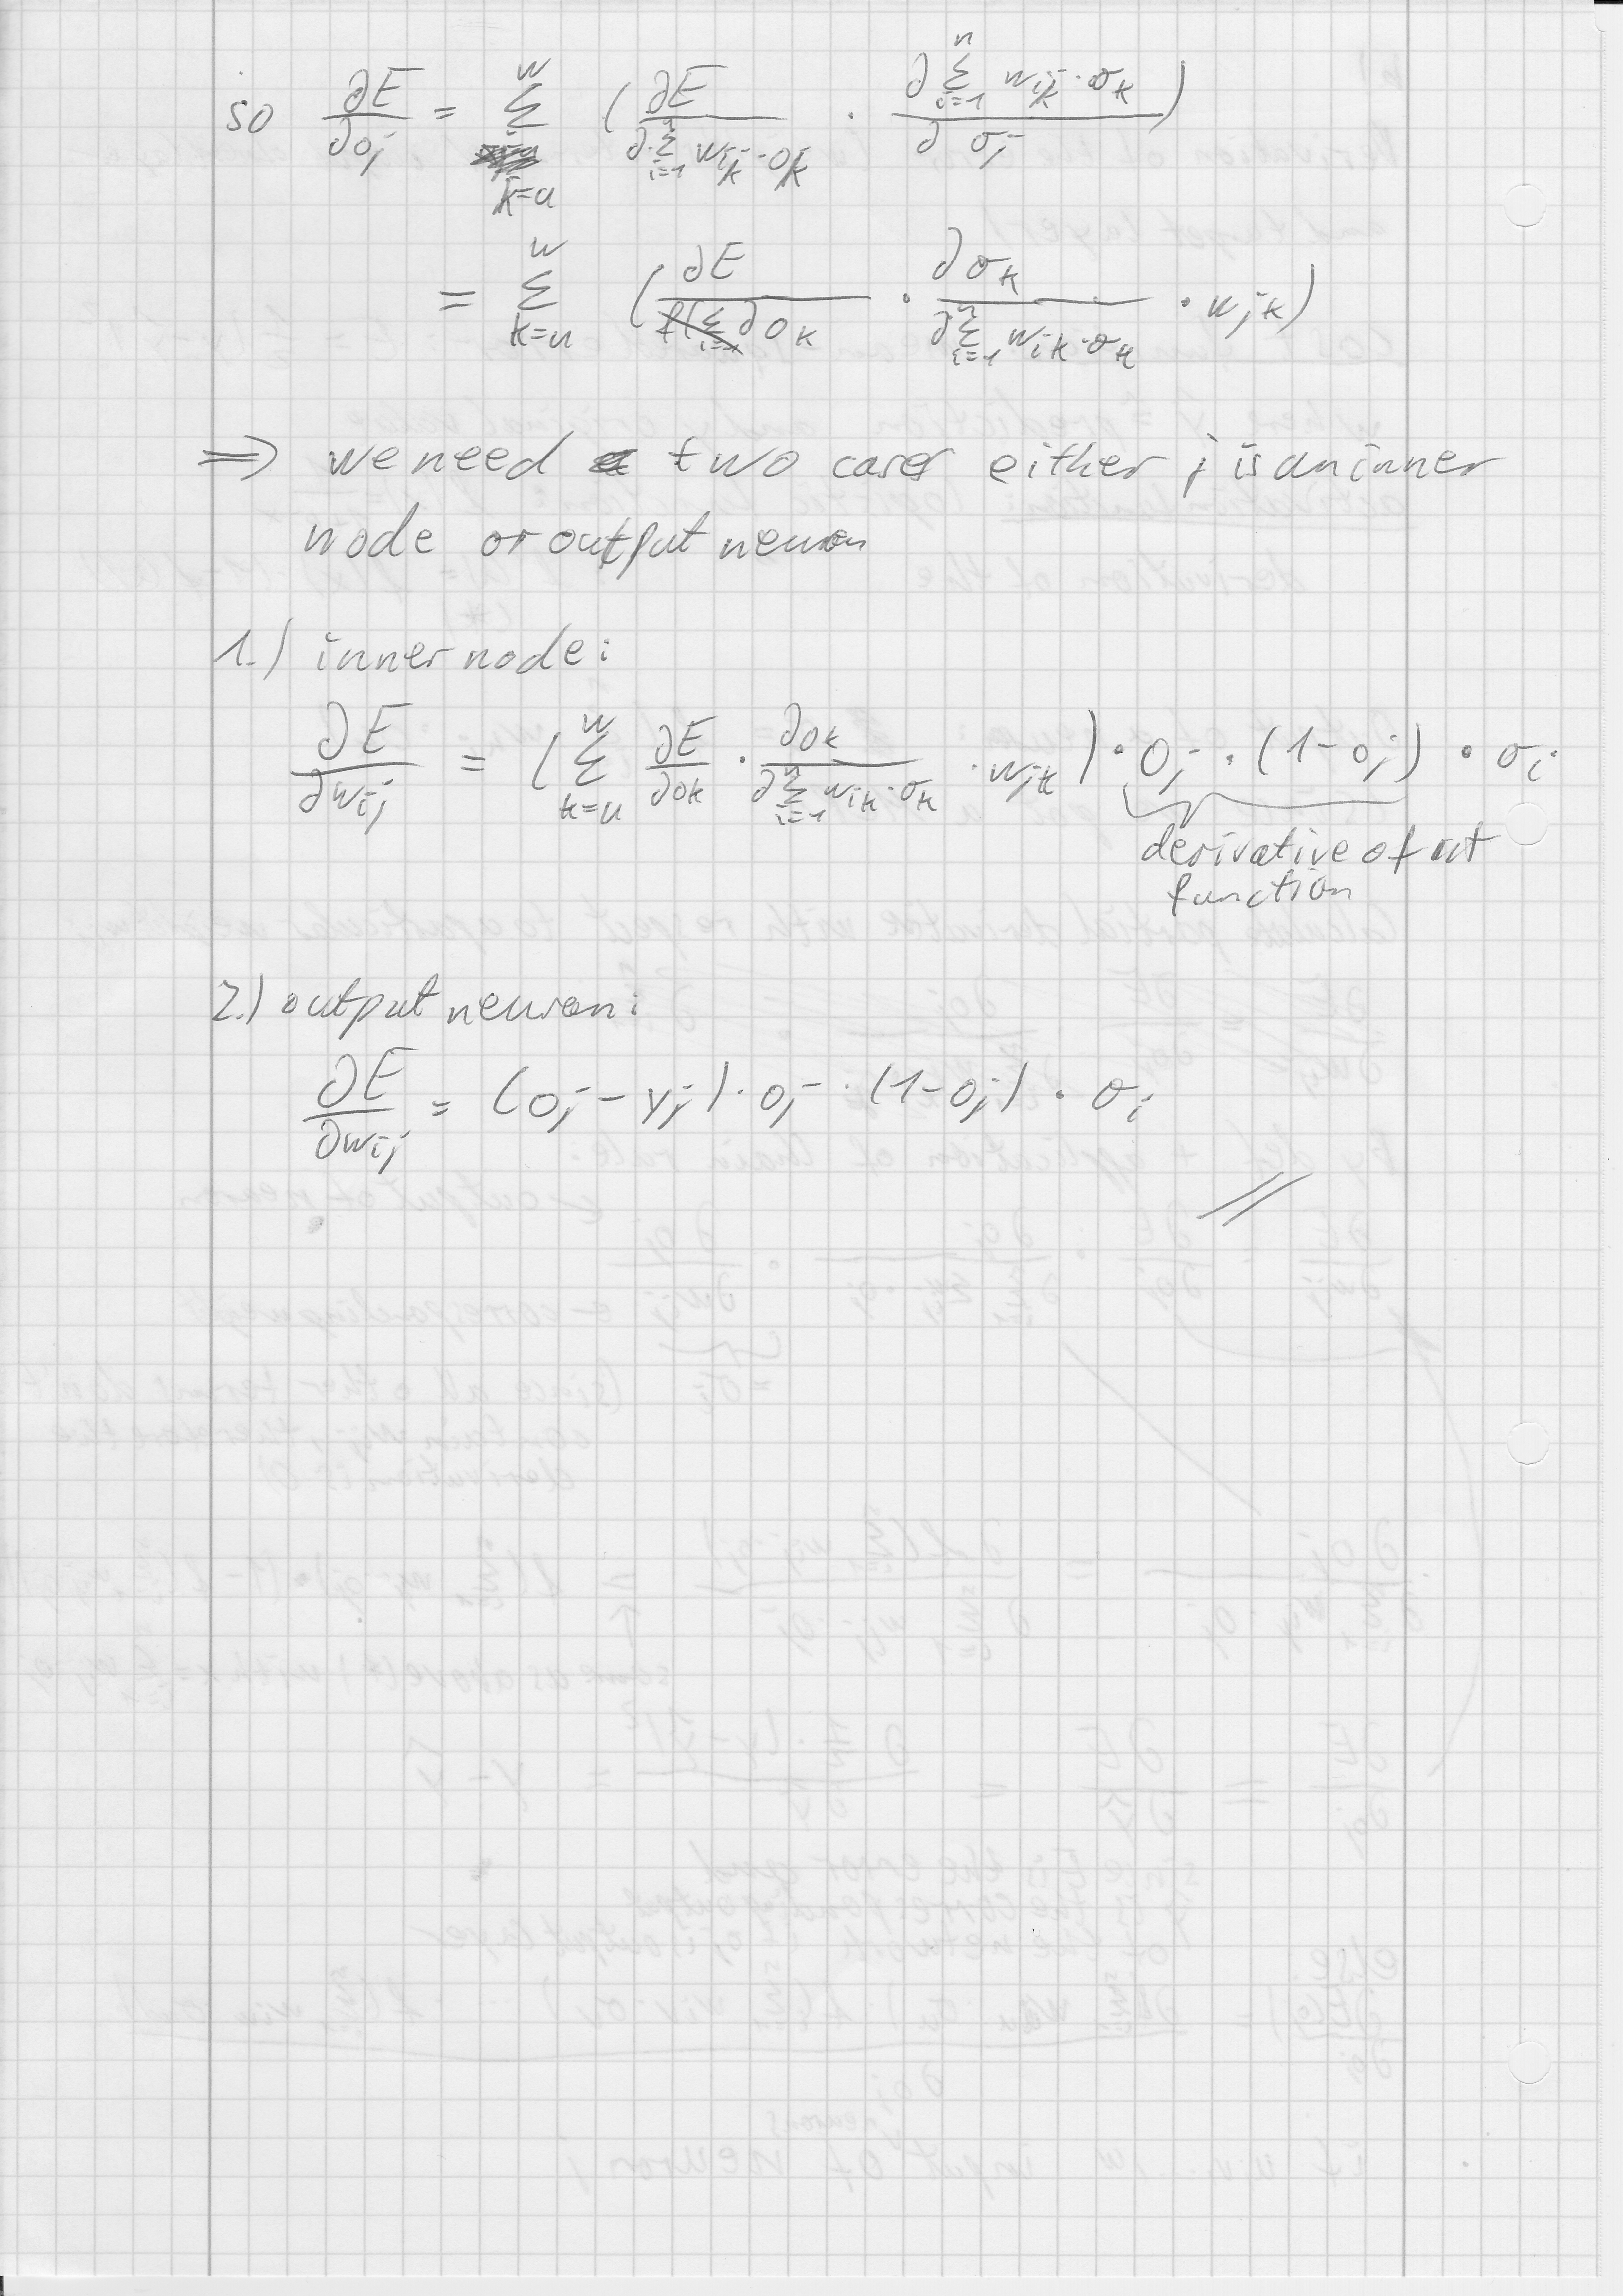
\includegraphics[scale = 0.1]{pictures/SCN_0002.jpg}\\
    \item
        without a non-linear activation function in the network, a NN, no matter how many layers it had, would behave just like a single-layer perceptron, because summing these layers would give you just another linear function.\\

        \newpage
        \includegraphics[scale = 0.35]{pictures/figure01}\\

        You can clearly see in the notes that I wrote above that $\hat{y}$ stays a linear combination of the 3 Inputs. That means that there exists a linear activation-funktions and weights such that the network below produces exactly the same result:\\

        \includegraphics[scale = 0.32]{pictures/figure02}\\

\end{enumerate}



\end{document}
